% vim: set ts=2 sw=2 noet spell:

\chapter{Theory}

\begin{figure}
	\centering
	\resizebox{\linewidth}{!}{
		\documentclass[tikz]{standalone}

\usepackage{roboto}
\usepackage{roboto-mono}
\usepackage{tikz}        % Pretty drawings
\usepackage{tikz-3dplot} % More dimensions!
\usetikzlibrary{
	external,
	calc,
	positioning,
	backgrounds,
	decorations.pathreplacing,
	calligraphy,
	decorations.markings,
	matrix,
	arrows,
	patterns,
}
\pgfdeclarelayer{background}
\pgfdeclarelayer{foreground}
\pgfsetlayers{background,main,foreground}

\begin{document}
\documentclass[tikz]{standalone}

\usepackage{roboto}
\usepackage{roboto-mono}
\usepackage{tikz}        % Pretty drawings
\usepackage{tikz-3dplot} % More dimensions!
\usetikzlibrary{
	external,
	calc,
	positioning,
	backgrounds,
	decorations.pathreplacing,
	calligraphy,
	decorations.markings,
	matrix,
	arrows,
	patterns,
}
\pgfdeclarelayer{background}
\pgfdeclarelayer{foreground}
\pgfsetlayers{background,main,foreground}

\begin{document}
\documentclass[tikz]{standalone}

\usepackage{roboto}
\usepackage{roboto-mono}
\usepackage{tikz}        % Pretty drawings
\usepackage{tikz-3dplot} % More dimensions!
\usetikzlibrary{
	external,
	calc,
	positioning,
	backgrounds,
	decorations.pathreplacing,
	calligraphy,
	decorations.markings,
	matrix,
	arrows,
	patterns,
}
\pgfdeclarelayer{background}
\pgfdeclarelayer{foreground}
\pgfsetlayers{background,main,foreground}

\begin{document}
\include{tikz/overview.tex}
\end{document}

\end{document}

\end{document}

	}
	\caption{
		Block diagram for a general wireless communication system with annotated signal names. Frequency domain representations of signals use the uppercase symbol of their respective time domain name.
		\label{fig:notation}
	}
\end{figure}

In this section we will briefly give the mathematical background required by the modulation schemes used in the project. The notation used is summarised in figure \ref{fig:notation}. For conciseness encoding schemes and (digital) signal processing calculations are left out and discussed later. Thus for this section \(m_e = m\).

%% TODO: Par on notation m(n) = m(nT) = discrete time

%% TODO: A section on maths?
% \section{Signal space and linear operators}

\section{Quadrature amplitude modulation (\(M\)-ary QAM)}

\begin{figure}
	\centering
	\resizebox{\linewidth}{!}{
		% vim: set ts=2 sw=2 noet:

\begin{circuitikz}[
	]
	\matrix [
		row sep = 5mm, column sep = 7mm,
		nodes = {
			align = center,
			fill = white,
		},
	] {
		& \coordinate (vmi);
			& \node[twoportshape] (B2Li) {};
			&
			& \coordinate (mi);
			&
			& \node[mixer] (Mi) {};
			& \coordinate (si);
			\\
		\node[] (M) {\(m(n)\)};
			& \node[twoportshape] (BSp) {};
			&
			&
			& \node[twoportshape] (H) {};
			& \node[oscillator] (OSC) {};
			& \coordinate (phii);
			& \node[adder] (SUM) {};
			& \node (S) {\(s(t)\)};
			\\
		&&&& \coordinate (phiq);
			\\[-3mm]
		& \coordinate (vmq);
			& \node[twoportshape] (B2Lq) {};
			& \coordinate (mq);
			& \node[mixer] (Mq) {};
			&
			&
			& \coordinate (sq);
			\\
	};

	% Add missing lables
	\node at (H.center) {\large \(\mathcal{H}\)};
	\node at (B2Li.center) {\textsf{B2L}};
	\node at (B2Lq.center) {\textsf{B2L}};
	\node at (BSp) {\textsf{BSp}};

	% Add connections
	\begin{scope}[thick, -latex]
		\draw (M) -- (BSp.west);

		\draw (BSp.north) |- (B2Li.west);
		\draw (B2Li.east) -- (Mi.west);
		\draw (Mi.east) -| (SUM.north);

		\draw (BSp.south) |- (B2Lq.west);
		\draw (B2Lq.east) -- (Mq.west);
		\draw (Mq.east) -| (SUM.south);

		\draw (SUM.east) -- (S);

		\draw (OSC.east) -| (Mi.south);
		\draw (OSC.west) -- (H.east);
		\draw (H.south) -- (Mq.north);
	\end{scope}

	% Add signal labels
	\node[above right] at (vmi) {\(\vec{m}_i\)};
	\node[below right] at (vmq) {\(\vec{m}_q\)};

	\node[above] at (mi) {\(m_i(t)\)};
	\node[below] at (mq) {\(m_q(t)\)};

	\node[above right] at (phii) {\(\phi_i\)};
	\node[right, yshift = 1mm] at (phiq) {\(\phi_q\)};

	\node[above left] at (si) {\(s_i(t)\)};
	\node[below left] at (sq) {\(s_q(t)\)};

	% Draw digital signals
	\begin{scope}[font = \ttfamily\footnotesize, text = blue!70!white]
		\node[above = 1mm of M, xshift = 2mm] {\(\ldots 1100101\)};
		\node[above = 7mm of vmi, xshift = 3mm]
			{\(\overbracket[.8pt]{\,11\ldots 00\,}^{\sqrt{M} \text{ bits}}\)};
	\end{scope}

	% Draw analog waveform
	\begin{scope}[font = \ttfamily\tiny]
		\coordinate (O) at ($(mi)+(-2mm,10.5mm)$);

		\node[left, red!70!white, anchor = east, text width = 8mm, align = right]
			at ($(O) + (-2mm,0)$) {\(2^{\sqrt{M}}\) levels};

		\foreach \y in {-3mm,0,3mm} {
			\draw[gray, densely dotted] (O) ++(-2mm,\y) -- ++(22mm,0);
		}

		\draw[thick, draw = red!70!white] (O)
			-- ++(3mm,0) -- ++(0,-3mm) -- ++(3mm,0) -- ++(0,6mm)
			-- ++(3mm,0) -- ++(0,-3mm) -- ++(3mm,0) -- ++(0,-3mm)
			-- ++(3mm,0) -- ++(0,3mm)  -- ++(3mm,0);
	\end{scope}

	% Draw constellation diagram
	\begin{scope}
		\coordinate (O) at ($(S)+(-7mm,8mm)$);
		\draw[gray, -latex] (O) ++(-2mm,0) -- ++(12mm,0) node[right] {\tiny \(\phi_i\)};
		\draw[gray, -latex] (O) ++(0,-2mm) -- ++(0,12mm) node[above] {\tiny \(\phi_q\)};

		\node[
			circle, thick,
			minimum size = 3pt,
			inner sep = 0, outer sep = .8pt,
			draw = gray, fill = red!50!white
		] (P) at ($(O)+(5mm, 4mm)$) {};

		\node[gray, above right] at (P) {\tiny \(s\)};

		\draw[gray, densely dotted]
			(P) -- (P |- O)
			(P) -- (P -| O);
	\end{scope}


	% Background elements
	\begin{pgfonlayer}{background}
		\fill[left color = white, right color = blue!20, draw = white]
			($(B2Li.north) + (0,1.1)$) coordinate (D) rectangle ($(B2Lq.south) - (3,1)$);
		\fill[right color = white, left color = red!20, draw = white]
			($(B2Li.north) + (0,1.1)$) coordinate (A) rectangle ($(B2Lq.south) + (9,-1)$);

		\node[blue!50, anchor = south east, font = \ttfamily\bfseries, xshift = -4mm]
			at (D) {\bfseries\ttfamily Digital bits};
		\node[red!50, anchor = south west, font = \bfseries\ttfamily, xshift = 4mm]
			at (A) {Analog waveform};
	\end{pgfonlayer}
\end{circuitikz}

	}
	\caption{
		Block diagram of a \(M\)-ary QAM modulator.
		\label{fig:quadrature-modulation}
	}
\end{figure}

Quadrature amplitude modulation is a family of modern digital modulation methods, that use an analog carrier signal. The simple yet effective idea behind QAM is to encode extra information into an orthogonal carrier signal, thus increasing the number of bits sent per unit of time \cite{Gallager,Kneubuehler,Mathis,Hsu}. A block diagram of the process is shown in figure \ref{fig:quadrature-modulation}.

%% TODO: Quick par on "we will dicusss M-Ary QAM, M is 2^something"

\subsection{Modulation of a digital message}

\paragraph{Bit splitter}

As mentioned earlier, quadrature modulation allows sending more than one bit per unit time. The first step to do it is to use a so called bit splitter, that converts the continuous bitstream \(m(n)\) into pairs of chunks of \(\sqrt{M}\) bits. The two bit vectors of length \(\sqrt{M}\), denoted by \(\vec{m}_i\) and \(\vec{m}_q\) in figure \ref{fig:quadrature-modulation}, are called in-phase and quadrature component respectively\cite{Hsu}. The reason will become more clear later.

\paragraph{Binary to level converter}

%% TODO: explain why gray code

Both bit vectors \(\vec{m}_i, \vec{m}_q \in \{0,1\}^{\sqrt{M}}\) are sent through a binary to level converter. It's purpose is to reinterpret the bit vectors as a numbers, usually in gray code, and to convert them into analog waveforms, which we will denote with \(m_i(t)\) and \(m_q(t)\) respectively. Mathematically the binary to level converter can be described as:
\begin{equation}
	m_i(t) = \text{Level}(\vec{m}_i) \cdot p(t),
\end{equation}
i.e. a pulse function\footnote{Typically a root raised cosine to optimize for bandwidth \cite{Hsu}.} \(p(t)\) scaled by the interpreted binary value, written here using a ``Level'' function. So at this point a level of each analog waveform is encodes \(\sqrt{M}\) bits per unit time, and there are two of such waveforms.


\paragraph{Mixer}

Having analog level signals, it is this now possible to mix them with radio frequency carriers. Because there are two waveforms, one might expect that two carrier frequencies are necessary, however this is not the case. The two component \(m_i(t)\) and \(m_q(t)\) are mixed with two different periodic signals \(\phi_i(t)\) and \(\phi_q(t)\) that have the same frequency \(\omega_c = 2\pi / T\). Why this is possible is explained in the next section.


\subsection{Orthogonality of carrier signals}

Before explaining how the two carrier signals are generated, we first need to discuss some important mathematical properties \(\phi_i\) and \(\phi_q\) need to have, in order to modulate two messages over the same frequency \(\omega_c\). The two carriers need to be \emph{orthonormal}\footnote{Actually orthogonality alone would be sufficient, however then the left side of \eqref{eqn:orthonormal-condition} would not equal 1, and an inconvenient factor would be introduced in many later equations \cite{Gallager,Hsu}.} to each other, mathematically this is expressed by the conditions
\begin{subequations} \label{eqn:orthonormal-conditions}
	\begin{align}
		\langle \phi_i, \phi_q \rangle
			&= \int_T \phi_i \phi_q^* \, dt
			= 0, \text{ and } \label{eqn:orthogonal-condition} \\
		\langle \phi_k, \phi_k \rangle
			&= \int_T \phi_k \phi_k^*  \,dt = 1,
			\text{ where } k \text{ is either } i \text{ or } q. \label{eqn:orthonormal-condition}
	\end{align}
\end{subequations}
Provided these rather abstract conditions, let's define a new signal 
\begin{equation}
	s = m_i\phi_i + m_q\phi_q.
\end{equation}
%% TODO: is this assumption correct?
Notice that assuming \(m_i\) and \(m_q\) are constant\footnote{This is an approximation assuming that the signal changes much slower relative to the carrier.} over the carrier's period \(T\),
\begin{align*}
	\langle s, \phi_i \rangle = \int_T s \phi_i^* \,dt
		&= \int m_i \phi_i \phi_i^* + m_q \phi_q \phi_i^* \,dt \\
		&= m_i \underbrace{\int_T \phi_i \phi_i^* \,dt}_{1}
			+ m_q \underbrace{\int_T \phi_q \phi_i^* \,dt}_{0} = m_i,
\end{align*}
which effectively means that it is possible to isolate a single component \(m_i(t)\) out of \(s(t)\). The same of course works with \(\phi_q\) as well resulting in \(\langle s, \phi_q \rangle = m_q\). Thus (remarkably) it is possible to send two signals on the same frequency, without them interfering with each other. Since each signal can represent one of \(\sqrt{M}\) values, by having two we obtain \(\sqrt{M} \cdot \sqrt{M} = M\) possible combinations.

A graphical way to see what is happening, is to observe a so called \emph{constellation diagram}. An example is shown in figure \ref{fig:qam-constellation} for \(M = 16\). The two carrier signals \(\phi_i\) and \(\phi_q\) can be understood as bases of a coordinate system.

\subsection{Construction of orthogonal carrier signals}


If \(\phi_i\) is a real valued signal (which is typical) it is possible to find a function the quadrature carrier using the \emph{Hilbert transform}:
\begin{equation}
	\hilbert g(t) = g(t) * \frac{1}{\pi t}
		= \frac{1}{\pi} \int_\mathbb{R} \frac{g(\tau)}{t - \tau} \,d\tau
		= \frac{1}{\pi} \int_\mathbb{R} \frac{g(t - \tau)}{\tau} \,d\tau,
\end{equation}
i.e. a linear operator that introduces a phase shift of \(\pi / 2\) over all frequencies \cite{Hsu,Gallager}. It is a known property of the Hilbert transform that given a real valued function \(g(t)\) then \(\langle g, \hilbert g \rangle = 0\) \cite{Kschischang,Kneubuehler}.
In practice \(\phi_i(t) = \cos(\omega_c t)\) and \(\phi_q(t) = \hilbert \phi_i(t) = \sin(\omega_c t)\).  

\paragraph{Oscillator and phase shifter}

\subsection{Spectral properties of a QAM signal}

\begin{figure}
	\hfill
	\begin{subfigure}{.4\linewidth}
		% vim: set ts=2 sw=2 noet:
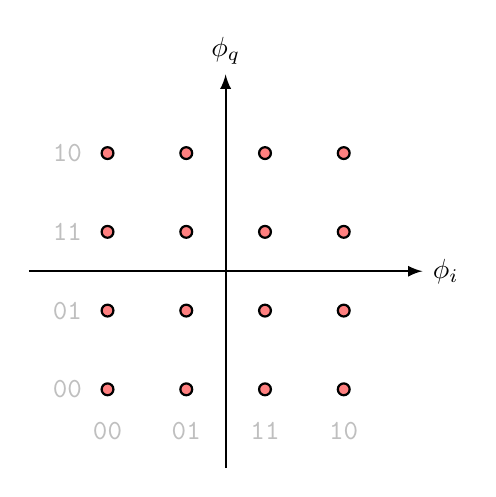
\begin{tikzpicture}[
		axis/.style = {
			thick, -latex, black,
		},
		star/.style = {
			draw = black, thick, fill = red!50,
			circle, outer sep = 1mm, inner sep = 0,
			minimum size = 1.5mm,
		},
	]
	\draw[axis] (-25mm,0) to (25mm,0) node[right] {\(\phi_i\)};
	\draw[axis] (0,-25mm) to (0,25mm) node[above] {\(\phi_q\)};

	\foreach \i in {0,1,...,3}{
		\foreach \q in {0,1,...,3}{
			\node[star] (s\i\q) at ({\i*10mm - 15mm},{\q*10mm - 15mm}) {};
		}
	}

	\foreach \i/\l in {0/00,1/01,2/11,3/10}{
		\node[lightgray, below = 3mm] at (s\i0) {\texttt{\l}};
		\node[lightgray, left = 2mm] at (s0\i) {\texttt{\l}};
	}
\end{tikzpicture}

		\caption{16-QAM\label{fig:qam-constellation}}
	\end{subfigure}
	\hfill
	\begin{subfigure}{.4\linewidth}
		\input{figures/tikz/psk-constellation}
		\caption{8-PSK\label{fig:psk-constellation}}
	\end{subfigure}
	\hfill
	\caption{
		Examples of constellation diagrams. Each dot represents a possible location for the complex amplitude of the passband signal.
	}
\end{figure}


\section{Phase shift keying (\(M\)-PSK)}

PSK is a popular modulation type for data transmission\cite{Meyer2011}. With a bipolar binary signal, the amplitude remains constant and only the phase will be changed with phase jumps of 180 degrees, which can be seen as a multiplication of the carrier signal with $\pm$ 1. That is alow known as binary phase shift keying.

% \begin{figure}
% 	% TODO: Better Image
% 	% https://sites.google.com/site/billmahroukelec675/bipolar-phase-shift-keying
% 	\includegraphics[width=5cm]{./image/BPSK2.png}
% \end{figure}

Two bits are modulated at ones with the same bandwidth as a 2-PSK so more informations are transmitted at the same time. \cite{Meyer2011}
%TODO: Image Signal Raum 
Most times there is noise and the points on the constellation diagram become a surface. 
If the surfaces overlap there will be a problem with decoding. 

\section{Wireless channel}

In the previous section, we discussed how the data is modulated and demodulated at the two ends of the transmission system. In this section we will discuss what happens between the sender and receiver when the modulated passband signal is transmitted wirelessly.

In theory because wireless transmission happens through electromagnetic radiation, to model a wireless channel one would need to solve Maxwell's equations for either the electric or magnetic field, however in practice that is not (analytically) possible. Instead what is typically done, is to model the impulse response of the channel using a geometrical or statistical model, parametrized by a set of coefficients that are either simulated or measured experimentally \cite{Gallager}.

In our model we are going to include an additive white Gaussian noise (AWGN) and a Rician (or Rayleighan) fading; both are required to model physical effects of the real world. The former in particular is relevant today, as it mathematically describes dense urban environments.

\subsection{Additive white Gaussian noise}

%% TODO: Discuss thermal stuff etc?

\subsection{Geometric multipath fading model}

The simplest way to understand the multipath fading, is to consider it from a geometrical perspective. Figure \ref{fig:multipath-sketch} is a sketch a wireless transmission system affected by multipath fading. The sender's antenna radiates an electromagnetic wave in the direction of the receiver (red line), however even under the best circumstances a part of the signal is dispersed in other directions (blue lines).

\begin{figure}
	\centering
	% vim: set ts=2 sw=2 noet:
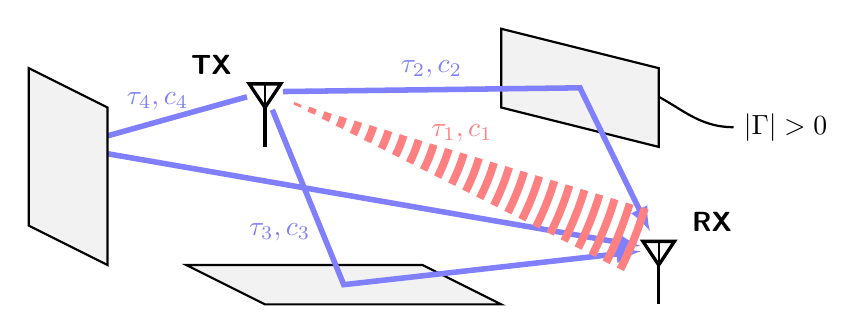
\begin{tikzpicture}[
			antenna/.pic = {
				\draw[very thick] (0,0) -- ++(2mm, 3mm) -- ++(-4mm,0) -- cycle;
				\draw[very thick] (0,0) -- ++(0,-5mm) coordinate (-mast) {};
				\draw[thick] (0,0) -- ++(0,3mm);
				\node[inner sep = 0pt, outer sep = 6pt] (-center) at (0,2mm) {};
			},
	]

	% Antennas
	\draw (0,2) pic (T) {antenna} node[above left = 3mm] {\sffamily\bfseries TX};
	\draw (5,0) pic (R) {antenna} node[above right = 3mm] {\sffamily\bfseries RX};

	% wall coefficients
	\draw[thick] (4.75, 2.25) to[out = -20, in = 180] ++(1.2,-.5) node[right] {\(|\Gamma| > 0\)};

	% walls
	\draw[thick, fill = lightgray!20] (3,2) -- ++(2,-.5) -- ++(0,1) -- ++(-2,.5) -- cycle;
	\draw[thick, fill = lightgray!20] (-1,0) -- ++(3,0) -- ++(1,-.5) -- ++(-3,0) -- cycle;


	% reflected signals
	\draw[line width = 2pt, blue!50!white, -latex] (T-center) -- node[above, pos = .5] {\(\tau_2,c_2\)} (4,2.25) -- (R-center);
	\draw[line width = 2pt, blue!50!white, -latex] (T-center) -- node[left, pos = .7] {\(\tau_3,c_3\)} (1,-.25) -- (R-center);
	\draw[line width = 2pt, blue!50!white, -latex] (T-center) -- node[above, pos = .5] {\(\tau_4,c_4\)} (-2.5,1.5) -- (R-center); 

	% another wall
	\draw[thick, fill = lightgray!20] (-2,0) -- ++(-1,.5) -- ++(0,2) --++(1,-.5) -- cycle;

	% LOS path
	\draw[line width = 1mm, red!50!white,
		decorate, decoration = {
			expanding waves, angle = 5, segment length = 2mm
		}
	] (T-center) -- node[above = 2mm, pos = .5] {\(\tau_1,c_1\)} (R-center);
\end{tikzpicture}

	\caption{
		Sketch of channel with multipath fading
		\label{fig:multipath-sketch}
	}
\end{figure}

The problem is that, as is geometrically evident, some paths are longer than others. Thus the signal is received by the receiver multiple times with different phase shifts \cite{Gallager,Messier}. To mathematically model this effect, we describe the received signal \(r(t)\) as a linear combination of delayed copies of the sent signal \(s(t)\), each with a different attenuation \(c_k\) and phase shift \(\tau_k\):
\begin{equation} \label{eqn:geom-multipath-rx}
	r(t) = \sum_k c_k s(t - \tau_k).
\end{equation}

The linearity of the model is justified by the assumption that the underlying electromagnetic waves behave linearly (superposition holds) \cite{Gallager}. How many copies of \(s(t)\) (usually referred to as ``taps'' or ``rays'') should be included in the formula, depends on the precision requirements of the model.

A further complication arises, when one end (or both) is not stationary. In that case the lengths of the paths change over time, and as a result both the delays \(\tau_k\) as well as the attenuations \(c_k\) become functions of time: \(\tau_k(t)\) and \(c_k(t)\) respectively \cite{Gallager,Messier}. Even worse is when the velocity at which the device is moving is high, because then Doppler shifts of the electromagnetic wave frequency become non negligible \cite{Gallager}.

We have thus observed that the arrangement can be modelled as a linear time-\emph{varying} system (LTV), if the sender or the receiver (or anything else in the channel) is moving, and as a linear time \emph{invariant} (LTI) system if the geometry is stationary. Regardless of which of the two cases, linearity alone is sufficient to approximate the channel as finite impulse response (FIR) filter \cite{Messier}. Mathematically we can rewrite LTV version of equation \eqref{eqn:geom-multipath-rx} using a convolution product as following:
\begin{align*}
	r(t) = \sum_k c_k(t) s(t - \tau_k(t)) &= \sum_k c_k(t) \int_\mathbb{R} s(\tau) \delta(\tau - \tau_k(t)) \,d\tau \\
		&= \int_\mathbb{R} s(\tau) \sum_k c_k(t) \delta(\tau - \tau_k(t)) \,dt' = s(\tau) * h(t, \tau),
\end{align*}
obtaining a new function
\begin{equation} \label{eqn:multipath-impulse-response}
	h(t,\tau) = \sum_k c_k(t) \delta(\tau - \tau_k(t)),
\end{equation}
that describes the \emph{impulse response} of the channel. This function is dependant on two time parameters: actual time \(t\) and convolution time \(\tau\). To better understand \(h(t,\tau)\), consider an example in shown in figure \ref{fig:multipath-impulse-response}. Each stem represents a weighted Dirac delta, so each series of stems of the same color, along the convolution time \(\tau\) axis, is a channel response at some specific time \(t\). Along the other \(t\) axis we see how the entire channel response changes over time\footnote{In the figure only a finite number of stems was drawn, but actually \(h(t,\tau)\) is continuous in \(t\), i.e. the weights \(c_k(t)\) of the Dirac deltas change continuously.}. Notice that the stems are not quite aligned to the \(\tau\) time raster (dotted lines), that is because in equation \eqref{eqn:multipath-impulse-response} not only the weights \(c_k\) but also the delays \(\tau_k\) are time dependent.

\begin{figure}
	\centering
	% vim: set ts=2 sw=2 noet:
\tdplotsetmaincoords{70}{40}
\begin{tikzpicture}[tdplot_main_coords, font = \footnotesize\ttfamily]
	\draw[thick, -latex] (0,0,0) -- node[sloped, midway, below, gray] {Effect of the channel} (7,0,0) node[right] {\(t'\)};
	\draw[thick, -latex] (0,0,0) -- node[sloped, midway, above, gray] {How the channel changes} (0,7,0) node[right] {\(t\)};
	\draw[thick, -latex] (0,0,0) -- (0,0,2) node[above] {\(h(t,t')\)};

	\foreach \y in {1,2,...,4}{
		\draw[dashed, gray] (0,1.5*\y,0) -- ++(7,0,0);
	}

	\foreach \x in {1,2,...,6}{
		\draw[dotted, gray] (\x,0,0) -- ++(0,7,0);
	}

	% draw 4 responses
	\begin{scope}[very thick, -{Circle[fill=white]}]
		\foreach \x/\v in {.8/1, 2.2/2, 2.9/1, 4/4, 5.1/7, 5.8/3}{
			\draw[blue!80!red] (\x,1.5*4,0) -- ++(0,0,\v/3);
		}

		\foreach \x/\v in {.9/2, 2.1/2, 3/1, 4/3, 5/6, 6/3}{
			\draw[blue!60!red] (\x,1.5*3,0) -- ++(0,0,\v/3);
		}

		\foreach \x/\v in {.6/1, 2/1, 2.8/3, 4.1/4, 5.5/4, 6.2/1}{
			\draw[blue!40!red] (\x,1.5*2,0) -- ++(0,0,\v/3);
		}

		\foreach \x/\v in {1.1/2, 1.8/1, 3/2, 3.7/1, 4.8/3, 5.8/1}{
			\draw[blue!20!red] (\x,1.5,0) -- ++(0,0,\v/3);
		}
	\end{scope}
\end{tikzpicture}

	\caption{
		LTV impulse response of a multipath fading channel.
		\label{fig:multipath-impulse-response}
	}
\end{figure}

\subsection{Spectrum of a multipath fading channel}

With a continuous time channel model we can now discuss the spectral properties of a fading channel. For this section, we will assume a LTI channel impulse response \(h(\tau)\) and consider a simple geometry.

\subsection{Discrete-time model}

\subsection{Statistical model}

%% TODO: write about advantage of statistical model instead of geometric

\section{Receiver DSP chain}
